%!TEX program=xelatex
\documentclass{article}
\usepackage{ctex}

% Set page size and margins
% Replace `letterpaper' with `a4paper' for UK/EU standard size
\usepackage[letterpaper,top=2cm,bottom=2cm,left=2.5cm,right=2.5cm,marginparwidth=1.75cm]{geometry}

% Useful packages
\usepackage{amsmath}
\usepackage{graphicx}
\usepackage{float}
\usepackage[colorlinks=true, allcolors=blue]{hyperref}

\title{微分方程数值解计算实习课后作业3}
\author{陈文宇}
\date{\today}


\begin{document}


\maketitle

\tableofcontents

\newpage
%---------------------------------------------------
\section{问题重述}

\begin{itemize}
    \item 画出数值解的图像
    \item 获取两类误差:
    $$ errL=(\int^{1}_{0}(\mu_{*}(x)-\mu_{n}(x))^{2}dx)^{\frac{1}{2}}$$
    $$ errH=(\int^{1}_{0}(\mu_{*}(x)-\mu_{n}(x))^{2}+(\mu'_{*}(x)-\mu'_{n}(x))^{2}dx)^{\frac{1}{2}}$$
    计算其关于网格长度的数值收敛阶
    \item 用$loglog()$函数展示$errL,errH,condA$的图像,
\end{itemize}
 
%---------------------------------------------------
\section{实验思路}
有限元方法求解:练习$2.1.1$
\[
\left\{
\begin{aligned}
	&-\mu '' + \frac{\pi^{2}}{4}\mu = \frac{\pi^{2}}{2}\sin{\frac{\pi}{2}x} \quad0<x<1 
	\\
	&\mu(0)=0 ,\quad \mu'(1)=0 
\end{aligned}
\right.
\]
对每个结点构造山形函数:对于i=1 2 ... n-1
\[
\phi_{i}(x)=
\left\{
\begin{aligned}
	&1+\frac{x+x_{i}}{h_{i}}   &x_{i-1}<x<x_{i}
	\\
	&1-\frac{x-x_{i}}{h_{i+1}} & x_{i}<x<x_{i+1}
        \\
        &  0 & \text{其他}
\end{aligned}
\right.
\quad
\phi_{n}(x)=
\left\{
\begin{aligned}
	&1+\frac{x+x_{n}}{h_{n}}   &x_{n-1}<x<x_{n}
	\\
        &  0 & \text{其他}
\end{aligned}
\right.
\]

考虑试探函数空间$U_{n}=\{\phi_{i}\}_{i=1}^{n}$,对任意$u_{h}\in U_{h}$可以表示为:
$$u_{n}=\sum_{i=1}^{n}u_{i}\phi _{i}(x),u_{i}=u_{h}(x_{i})$$

形成有限元方程后,求解线性方程组$Ax=b$即可获得基函数系数。
对于条件数可以使用matlab命令$cond(A,2)$,
定义errL和errH后,给出其离散点集,然后可以使用复化Simpson方法来求积分,
进而使用$plot,loglog$函数绘制图像即可。

\newpage
matlab编程的具体操作如下:
\begin{figure}[H]
\centering
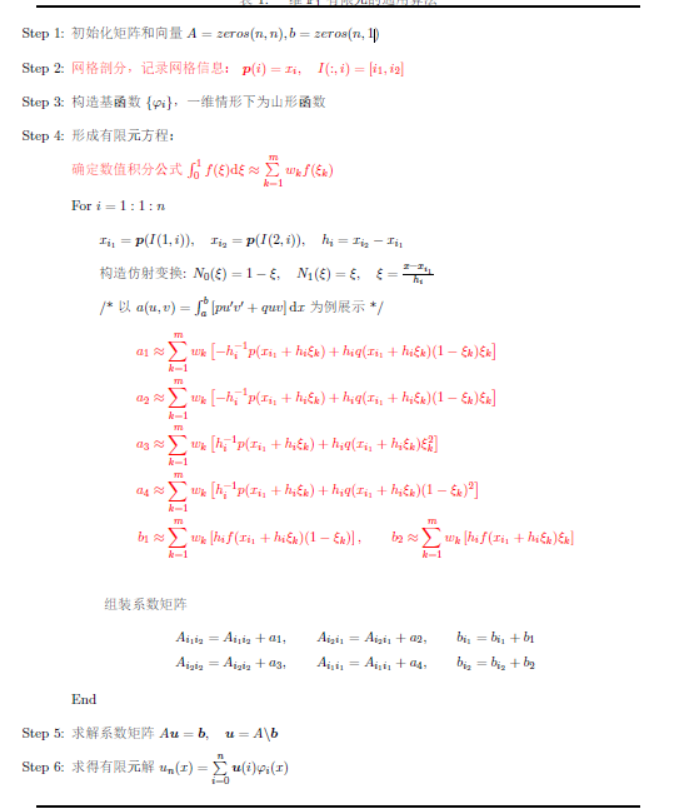
\includegraphics[scale=1.2]{Steps.png}
\end{figure}

\newpage
%---------------------------------------------------
\section{实验结果}

下图是数值解和精确解的图像:
\begin{figure}[H]
\centering
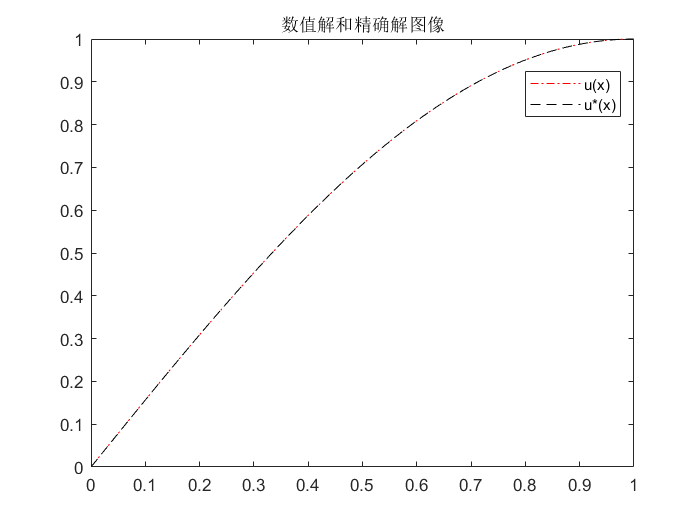
\includegraphics[scale=0.6]{Numerical solution image.png}
\caption{\label{Numerical solution image}数值解和精确解的图像}
\end{figure}

下图是$(logh,log(errL))$的图像,根据线性基本拟合,知$errL$收敛阶为2.
\begin{figure}[H]
\centering
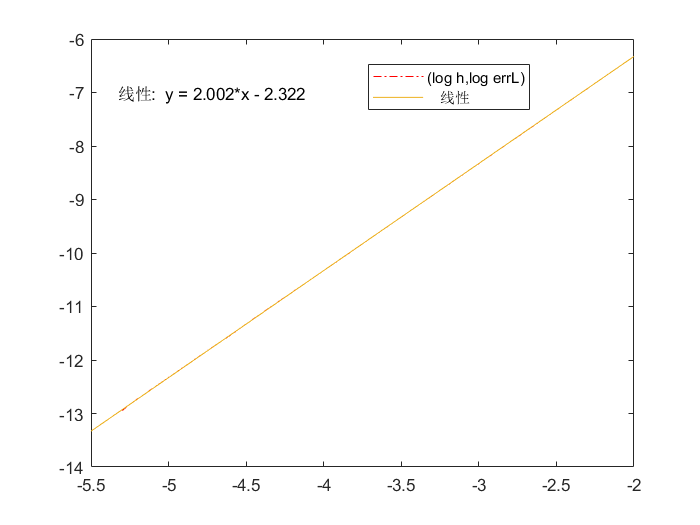
\includegraphics[scale=0.6]{errL_Convergence_Step.png}
\caption{\label{errL_Convergence_Step}$L^{2}([0,1])$误差的收敛阶}
\end{figure}

\newpage
下图是$(logh,log(errH))$的图像,根据线性基本拟合,知$errH$收敛阶为1.
\begin{figure}[H]
\centering
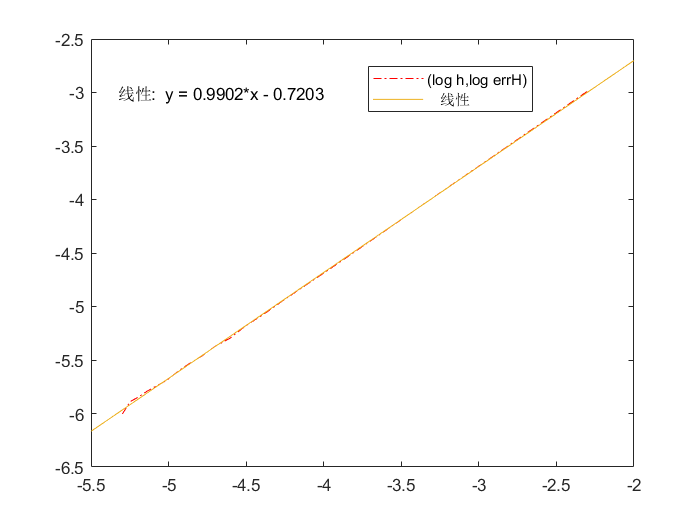
\includegraphics[scale=0.6]{errH_Convergence_Step.png}
\caption{\label{errH_Convergence_Step}$H^{1}([0,1])$误差的收敛阶}
\end{figure}

下面用$loglog()$函数展示$(h,errL),(h,errH)$。
\begin{figure}[H]
\centering
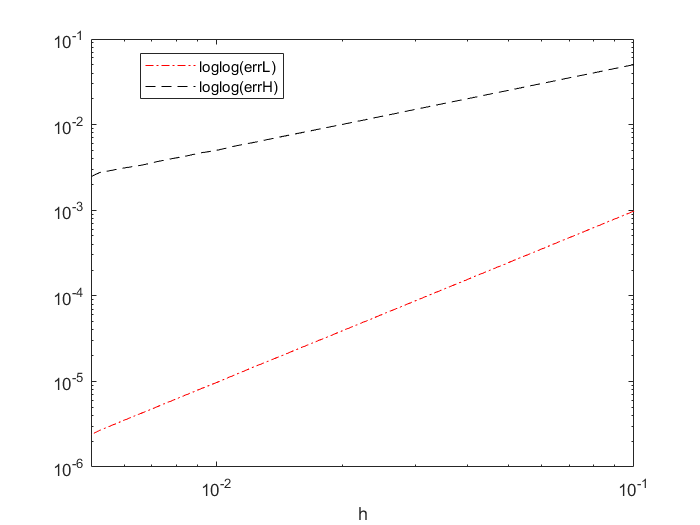
\includegraphics[scale=0.6]{loglog_err.png}
\caption{\label{loglog_err}$loglog_err$图像}
\end{figure}

\newpage
用$loglog()$函数展示矩阵A的条件数的变化。
\begin{figure}[H]
\centering
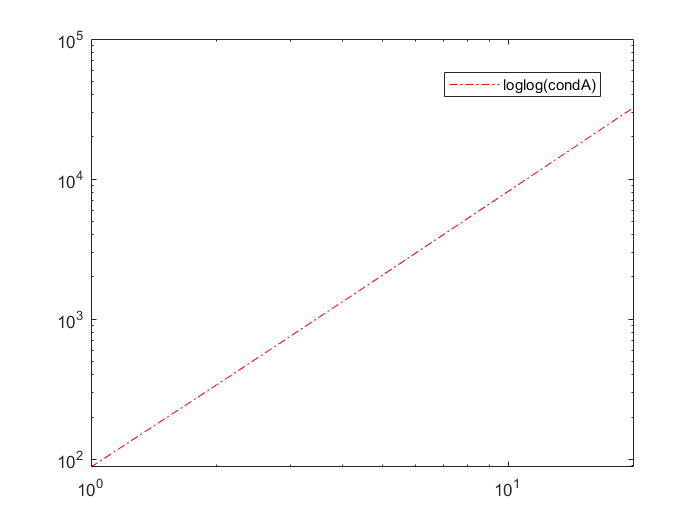
\includegraphics[scale=0.5]{loglog_condA.png}
\caption{\label{loglog_condA}$loglog_condA$}
\end{figure}


%-----------------------------------------------------
\section{实验结果分析}
对于本题,$errL$ 误差的收敛阶均为2,$errH$ 误差的收敛阶均为1,两类误差的收敛阶不同,可能是基函数为山形函数,其导数是阶梯函数,同原函数的导数误差较大造成的,不过可以猜测得到的是,随着区间剖分越来越细密,二者导数造成的误差会收敛于0。

根据矩阵A的定义,矩阵A是严格对角占优的,故而矩阵A是非奇异的矩阵。但是随着基函数的增加,矩阵A的对角占优的性质越来越弱,它的影响需要更多的精力来分析了。对于N=10:10:200,矩阵A的条件数增长,但并不趋向于极大,,求解方程$Ax=b$是稳定的,由下列图象知,condA 随 h 指数级增长。

\begin{figure}[H]
	\centering
	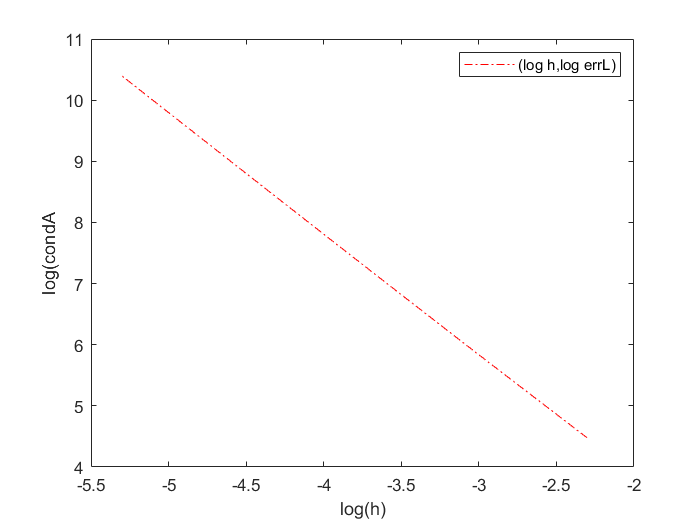
\includegraphics[scale=0.5]{logh_logcondA.png}
	\caption{\label{logh_logcondA}$logh_logcondA$}
\end{figure}




\end{document}